\documentclass[12pt,twoside]{article}

%%%%%%% Loading packages and macros %%%%%%%
\usepackage{preamble/__packages__}
\usepackage{preamble/__macro__}
%%%%%%%%%%%%%%%%%%%%%%%%%%%%%%%%%%%%%%%%%%%

%%%%%%% Document %%%%%%%
\newcommand{\assignment}{ssignment 6 }
\newcommand{\course}{FINC 585-3: Asset Pricing}
\newcommand{\prof}{Torben Andersen}
\newcommand{\institute}{Kellogg School of Management}

\title{\course-\assignment}
\author{TA: Jose Antunes-Neto}
\date{\today}
%%%%%%%%%%%%%%%%%%%%%%%%

\begin{document}
\maketitle

Our final Assignment concerns measurement of the (unconditional) Variance Risk Premium. For this purpose, you need to compute the realized volatility (RV) over the same period as the traditional VIX refers to, namely 30 (calendar) days. The most critical point is to include the squared overnight (or close-to-open) return for the S\&P 500 index in computing the RV. The ``overnight return” uses the increment in the log-price between the prior market close and the subsequent market open. An alternative is to estimate the average overnight squared return relative to the intraday RV and then scale up the intraday RV for a given day with the ratio of [average (intraday RV + squared overnight return) / average intraday RV]. We use the first approach below.

\begin{enumerate}[label = \arabic*)]
    \item Go back to the daily RV series for the spider that you computed in the last assignment based on returns sampled at a 5-minute frequency. Compute the mean for the daily RV series, where you express the mean value in terms of the daily squared percentage annualized value. Note that this computation involves only the high-frequency returns within the trading day (so any squared return overnight is ignored). Please assume there are 252 trading days per year when you annualize the trading day RV measure.
    
    \begin{solution}
        I calculate the Realized Volatility during the trading hours by summing the squared returns observed at the 5-minute frequency. The returns are annualized and shown in percentage. The SPY log-returns and the RV estimates are shown in Figure~\ref{fig:spy}. This is equivalent to the one that we did in the previous assignment. The average daily RV is 384.65\%
        \begin{figure}[!htbp]
            \centering
            \caption{5-Minute SPY returns and variance}
            \label{fig:spy}
            \begin{subfigure}[b]{0.45\textwidth}
              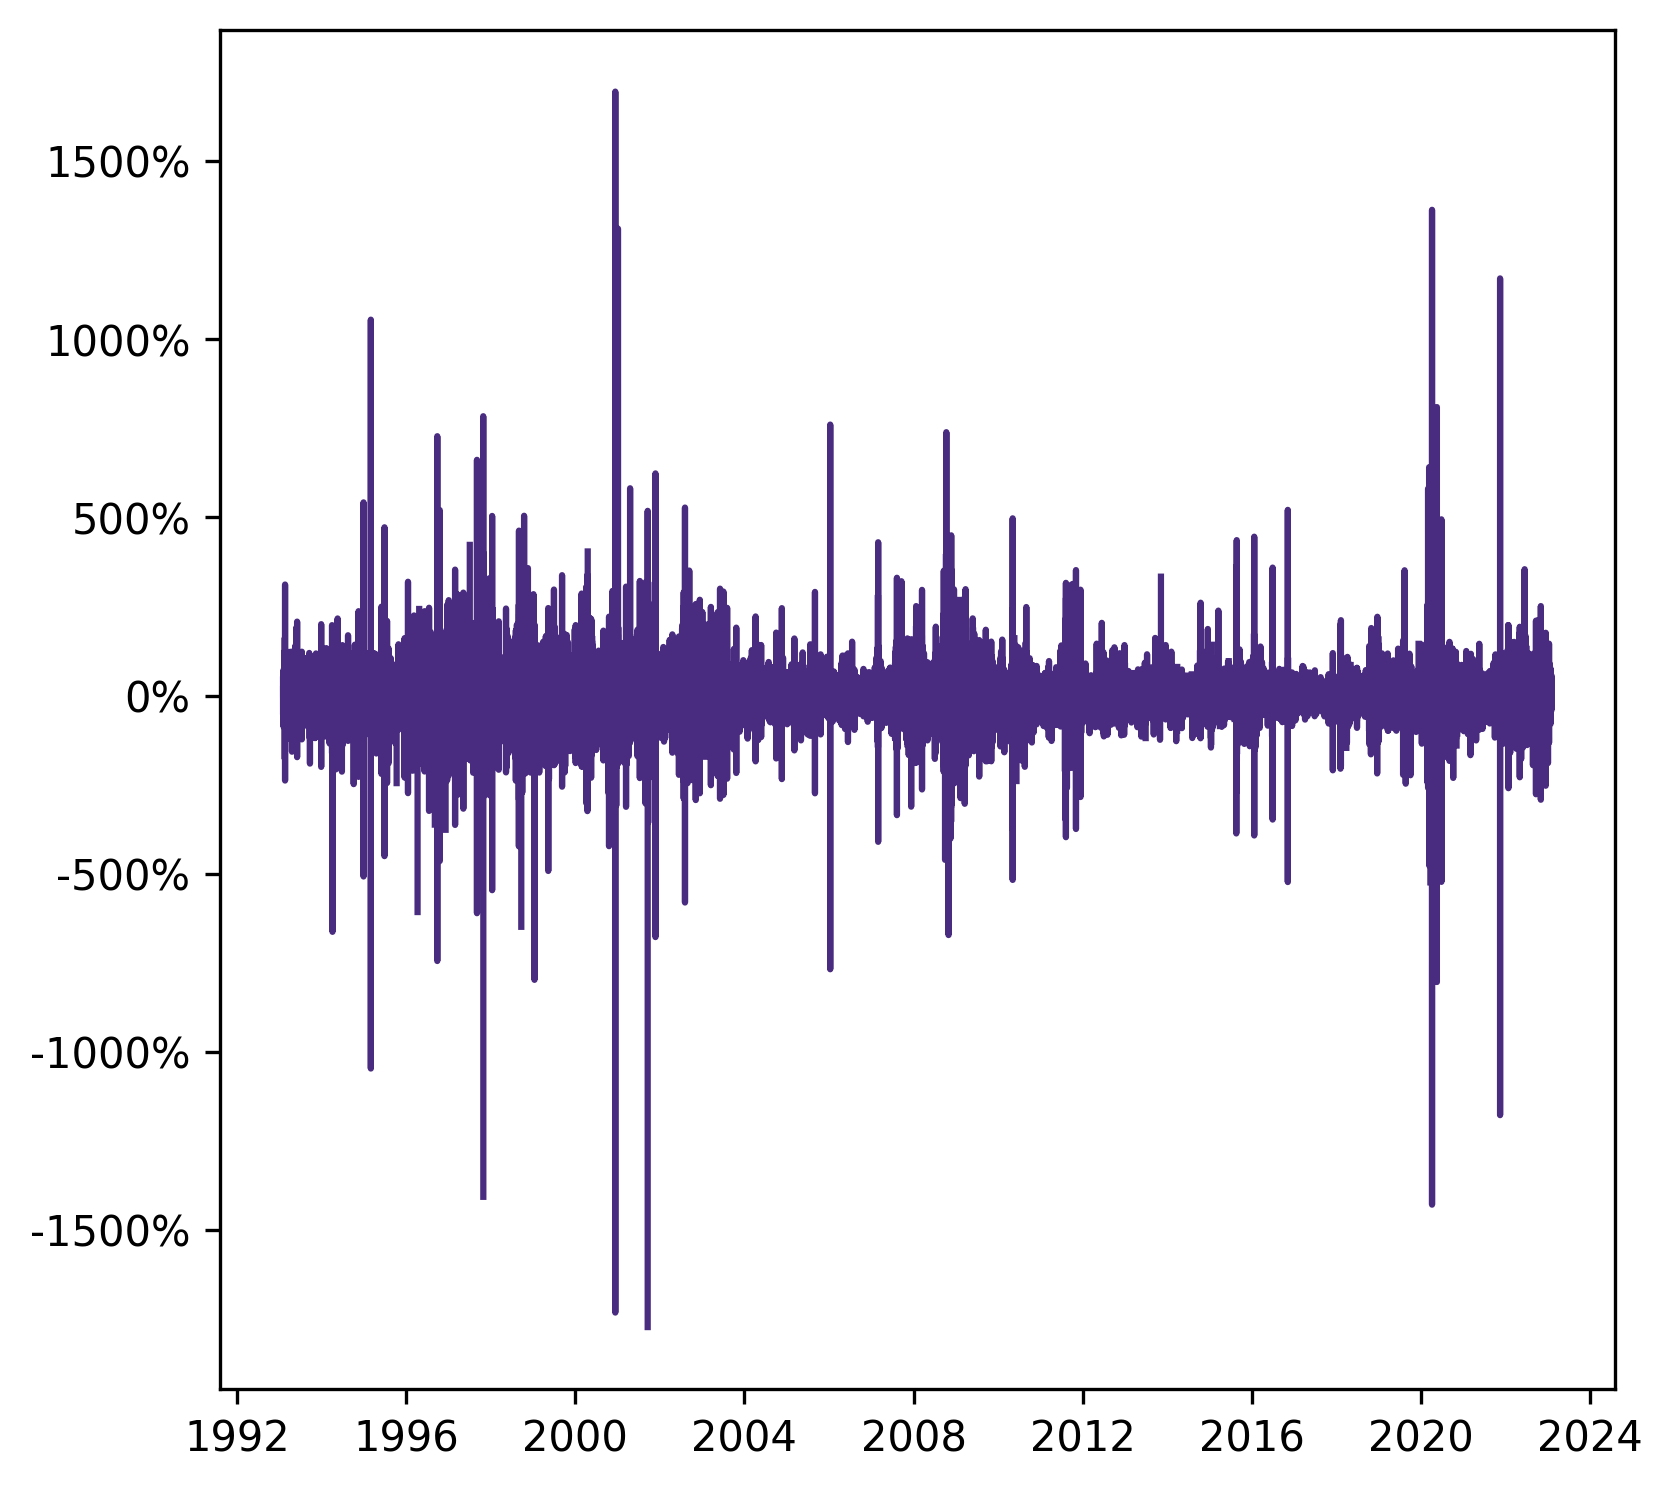
\includegraphics[width=\textwidth]{images/spy_returns.png}
              \caption{SPY 5-Minute Log-Returns}
              \label{fig:spy_returns}
            \end{subfigure}
            \hfill
            \begin{subfigure}[b]{0.45\textwidth}
              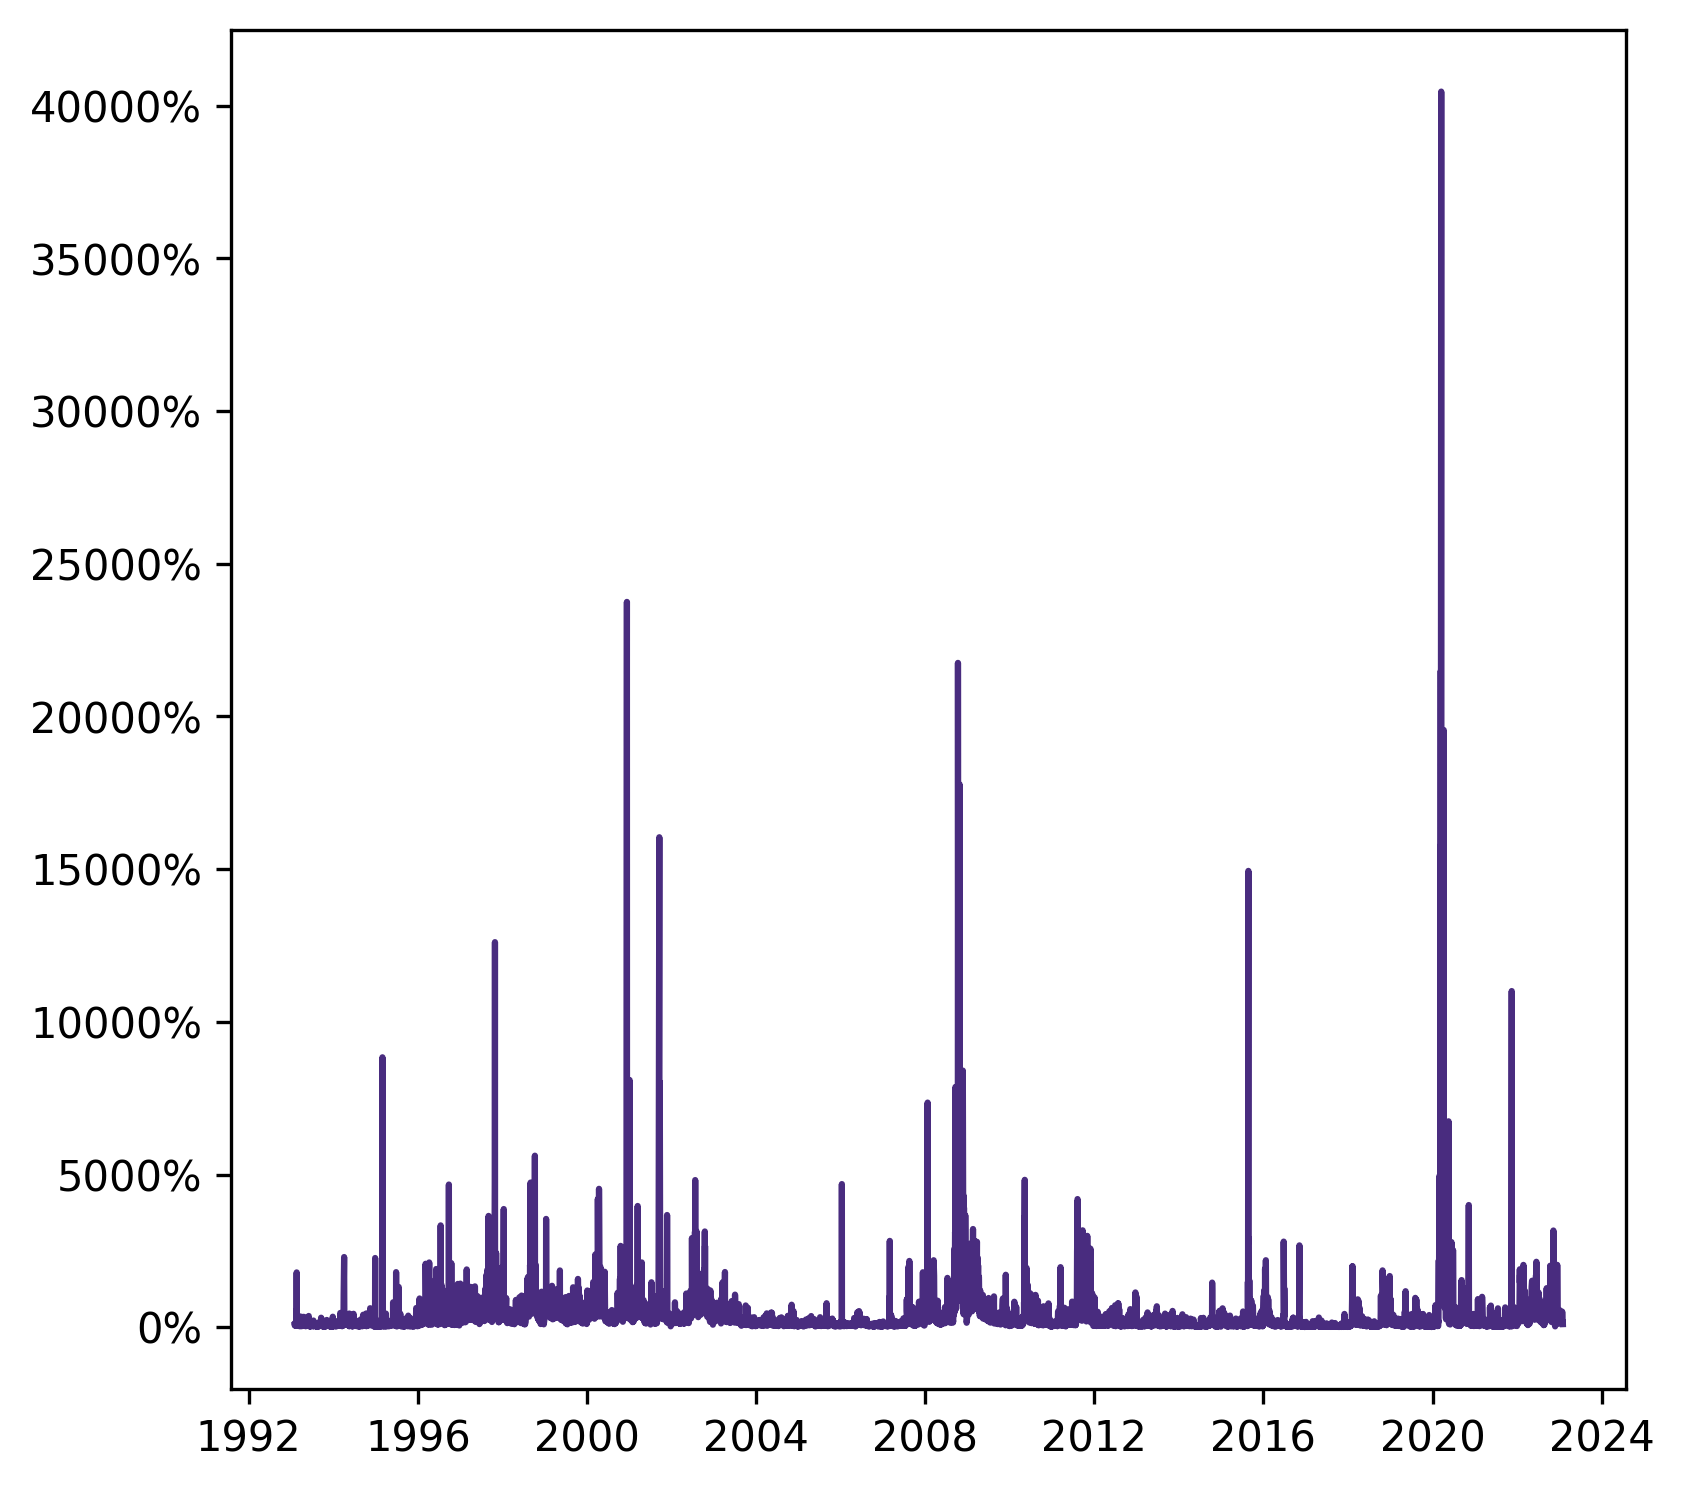
\includegraphics[width=\textwidth]{images/trading_rv.png}
              \caption{Realized Variance}
              \label{fig:trading_rv}
            \end{subfigure}
          \end{figure}
    \end{solution}

    \item Repeat the computation in question 1), but after adding the preceding squared overnight return to the RV. In this manner, the daily RV includes the cumulative squared returns for the trading day \textbf{plus} the squared return over the \textbf{preceeding} non-trading period.
    
    \begin{solution}
        To include the overnight realized volatility, I sample the observations on a daily frequency and calculate the market open and close price. The overnight realized volatility is then calculated as 
        \[
            Overnight\_RV \coloneqq \left(\text{Open}_t - \text{Close}_{t-1}\right)^2
        \]
        Adding it to the trading-hours RV makes significant changes to the series as shown in Table~\ref{tab:rv_stats}
        
        \begin{table}[!htbp]
            \centering
            \caption{Descriptive Statistics for the RV Series}
            \label{tab:rv_stats}
            \begingroup
            \color{nu purple}
            \begin{tabular}{lrrr}
\toprule
{} &        RV &  Overnight RV &  Total RV \\
\midrule
count &  7554.00\% &      7554.00\% &  7554.00\% \\
mean  &   384.69\% &        95.23\% &   479.92\% \\
std   &  1037.97\% &       604.58\% &  1551.00\% \\
min   &     4.34\% &         0.00\% &     4.62\% \\
25\%   &    76.96\% &         0.09\% &    88.76\% \\
50\%   &   170.52\% &         8.54\% &   199.20\% \\
75\%   &   373.89\% &        47.90\% &   436.60\% \\
max   & 40461.93\% &     34116.31\% & 74578.24\% \\
\bottomrule
\end{tabular}

            \endgroup
        \end{table}
    \end{solution}

    \item Now download the daily closing values for the VIX series from the Cboe website for historical VIX data. Note that these values are designed to reflect the square-root of the annualized 30-day expected return variation (RV) for the S\&P 500. \\
    Using the period of overlap between your RV series in question 2) and the VIX series, compute the average square-root of the 30 calendar-day annualized RV measure. What is the difference between this value and the average VIX computed over the full sample? This value is our simple estimate of the Volatility (square-root of variance) Risk premium. Computing the same differential between the corresponding RV and VIX2 series yields an estimate of the Variance Risk Premium.

    \begin{solution}
        The volatility risk premium corresponds to the negative returns of the variance swap contracts, which go long in the Realized Volatility (\(\sqrt{RV}\)) and pays VIX at maturity. Since the VIX corresponds to the expected realized volatility of the next 30 days, it is important to compare it to the 30-day \textbf{future} realized volatility. For this I calculate the 30-day moving average of the \emph{Total RV} series and compare it to the VIX 30 days ago. The volatility The descriptive statistics for the are shown in Table~\ref{tab:vol_premium_stats}. The results for the variance risk premium (\(\text{RV}-\text{VIX}^2\)) are shown in Table~\ref{tab:var_premium_stats}.
        \begin{table}[!htbp]
            \centering
            \caption{Descriptive Statistics for the VIX and \(\sqrt{\text{RV}}\)}
            \label{tab:vol_premium_stats}
            \begingroup
            \color{nu purple}
            \begin{tabular}{lrrr}
\toprule
{} &  Total RV &      VIX &  Volatility Risk Premium \\
\midrule
count &  7554.00\% & 7558.00\% &                 7521.00\% \\
mean  &    17.35\% &   19.76\% &                    2.39\% \\
std   &    13.38\% &    8.23\% &                    6.61\% \\
min   &     2.15\% &    9.14\% &                  -69.83\% \\
25\%   &     9.42\% &   13.68\% &                    0.53\% \\
50\%   &    14.11\% &   17.96\% &                    3.05\% \\
75\%   &    20.89\% &   23.39\% &                    5.39\% \\
max   &   273.09\% &   82.69\% &                   36.07\% \\
\bottomrule
\end{tabular}

            \endgroup
        \end{table}
        \begin{table}[!htbp]
            \centering
            \caption{Descriptive Statistics for the VIX and RV}
            \label{tab:var_premium_stats}
            \begingroup
            \color{nu purple}
            \begin{tabular}{lrrr}
\toprule
{} &  Total RV &      VIX &  Variance Risk Premium \\
\midrule
count &  7554.00\% & 7558.00\% &               7521.00\% \\
mean  &   479.92\% &  458.21\% &                -22.59\% \\
std   &  1551.00\% &  492.69\% &                720.23\% \\
min   &     4.62\% &   83.54\% &             -10403.05\% \\
25\%   &    88.76\% &  187.14\% &                -34.39\% \\
50\%   &   199.20\% &  322.74\% &                 57.17\% \\
75\%   &   436.60\% &  546.98\% &                141.96\% \\
max   & 74578.24\% & 6837.64\% &               4059.24\% \\
\bottomrule
\end{tabular}

            \endgroup
        \end{table}
    \end{solution}

    \item Plot the annualized percentage VIX and square-root RV series over the full sample period of overlap for the two series.
    \begin{solution}
        Finally, I plot the two series in Figure~\ref{fig:rv_and_vix}. We can see that the gap between them is consistent and higher in the most volatilite periods. Figure~\ref{fig:vol_premium} shows the result for the difference between the two series.

        \begin{figure}[!htbp]
            \begin{small}
                \begin{center}
                    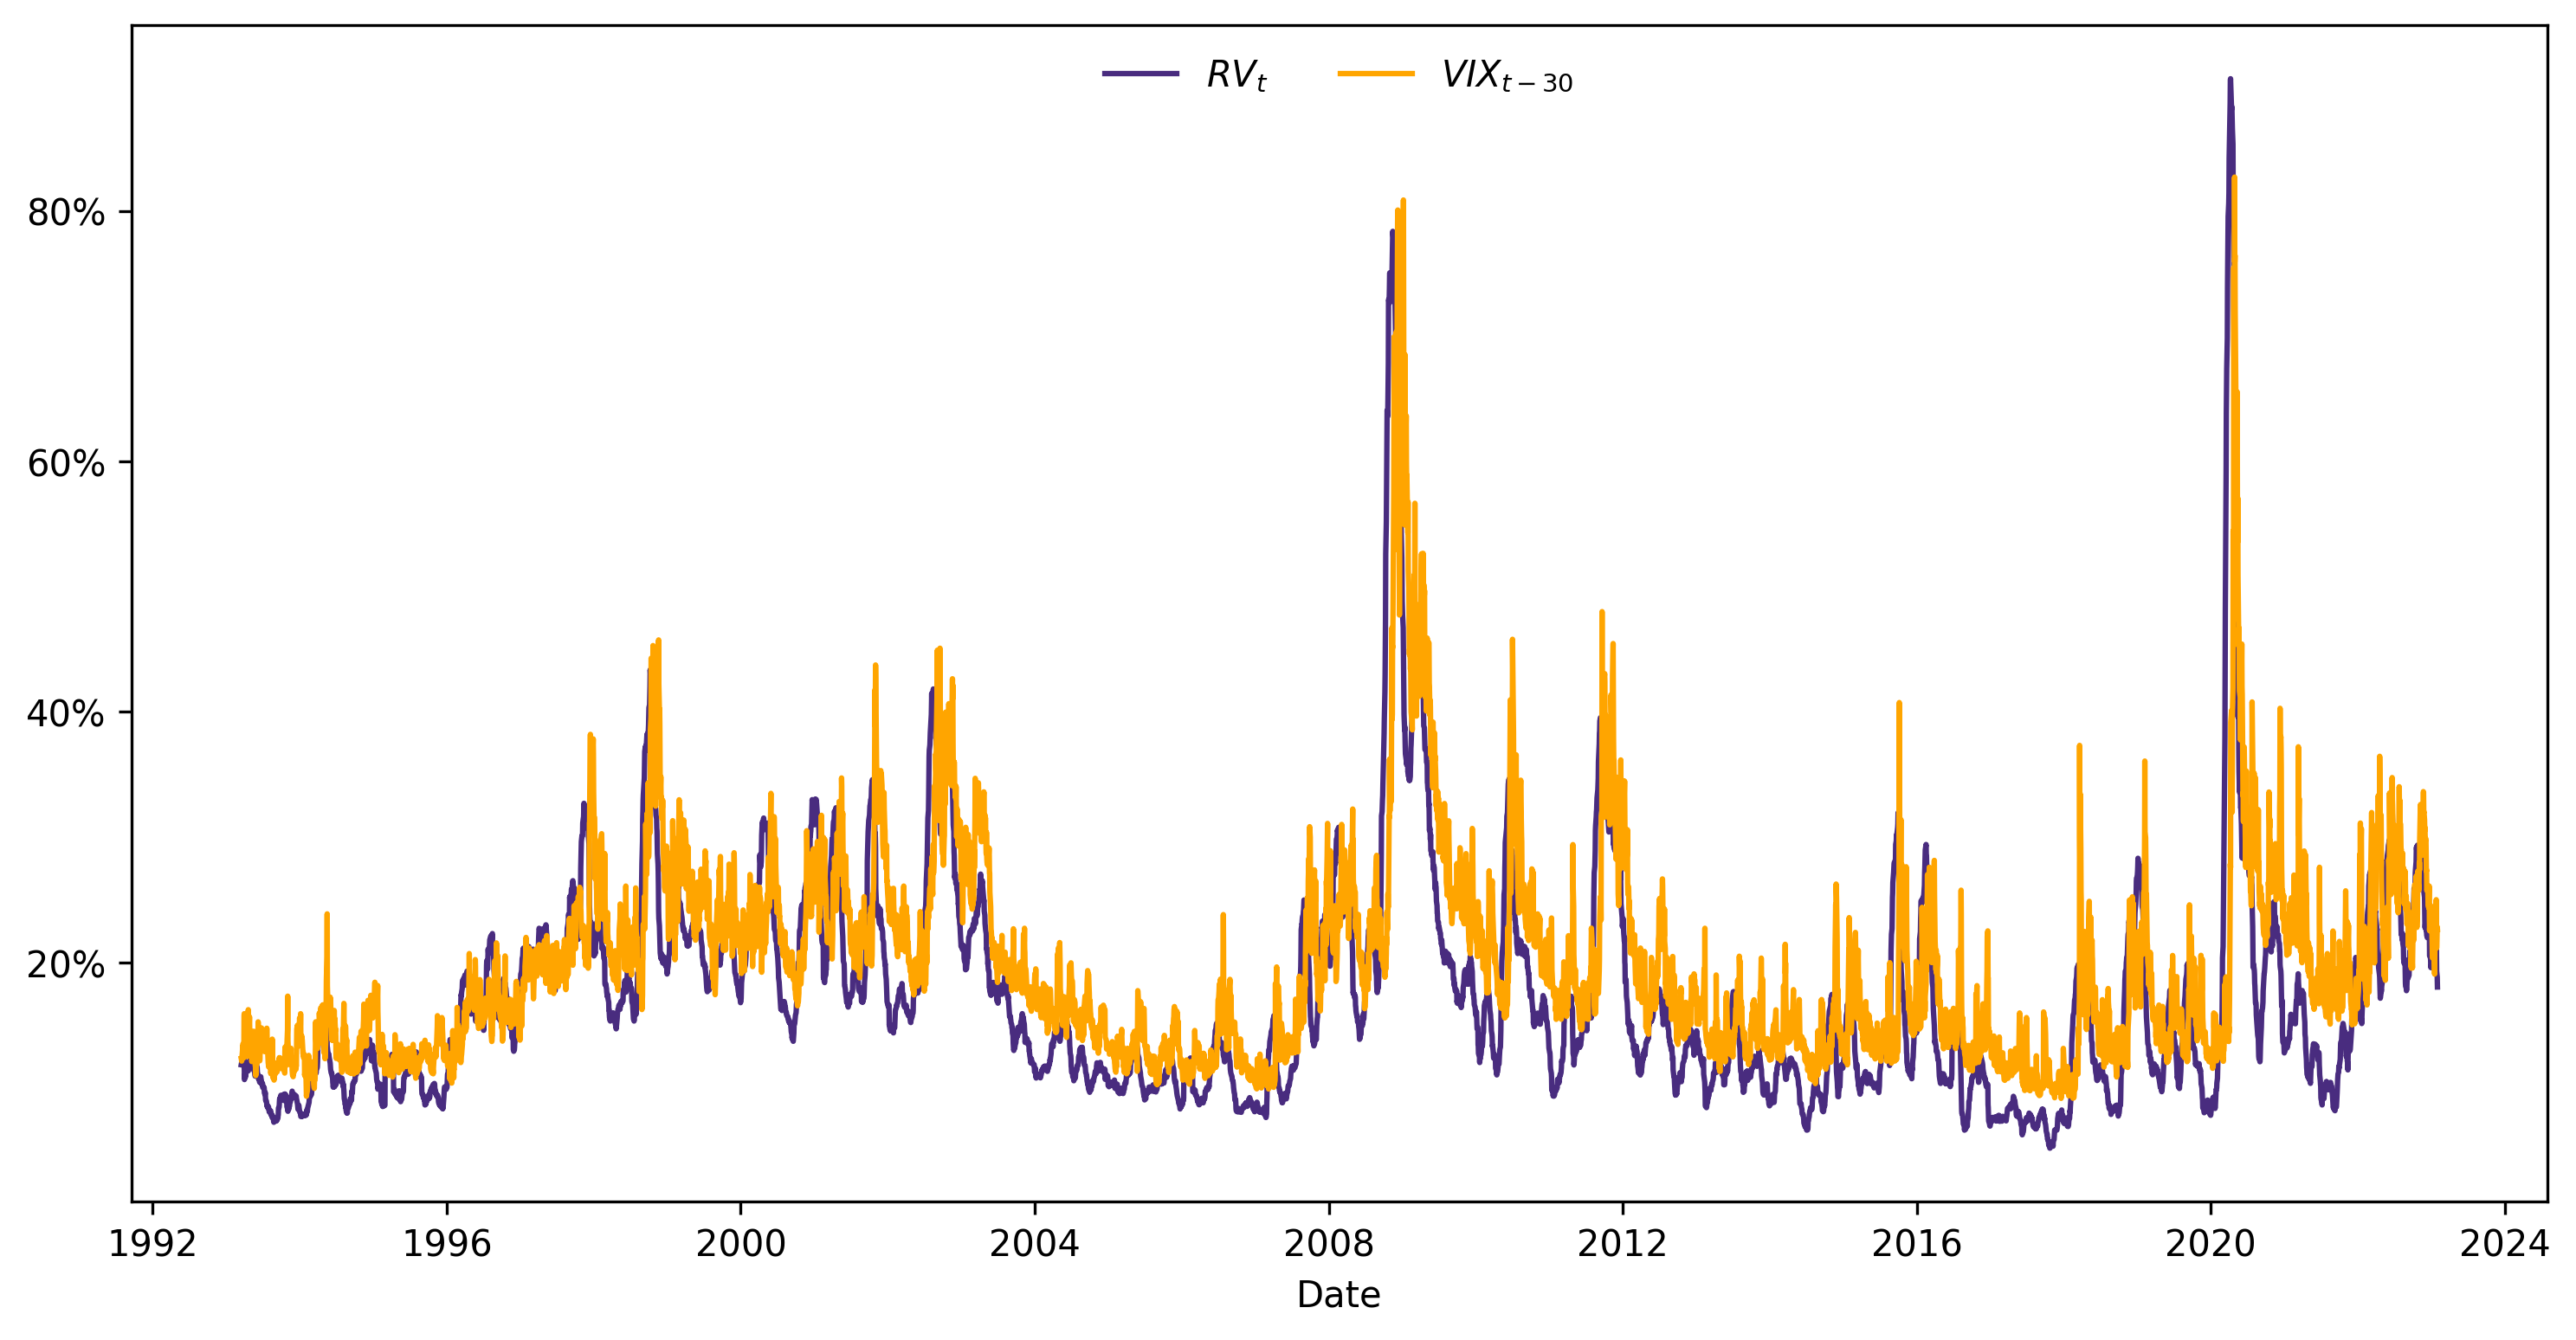
\includegraphics[width=0.95\textwidth]{images/rv_and_vix.png}
                \end{center}
                \caption{VIX and Realized Volatility}
                \label{fig:rv_and_vix}
            \end{small}
        \end{figure}

        \begin{figure}[!htbp]
            \begin{small}
                \begin{center}
                    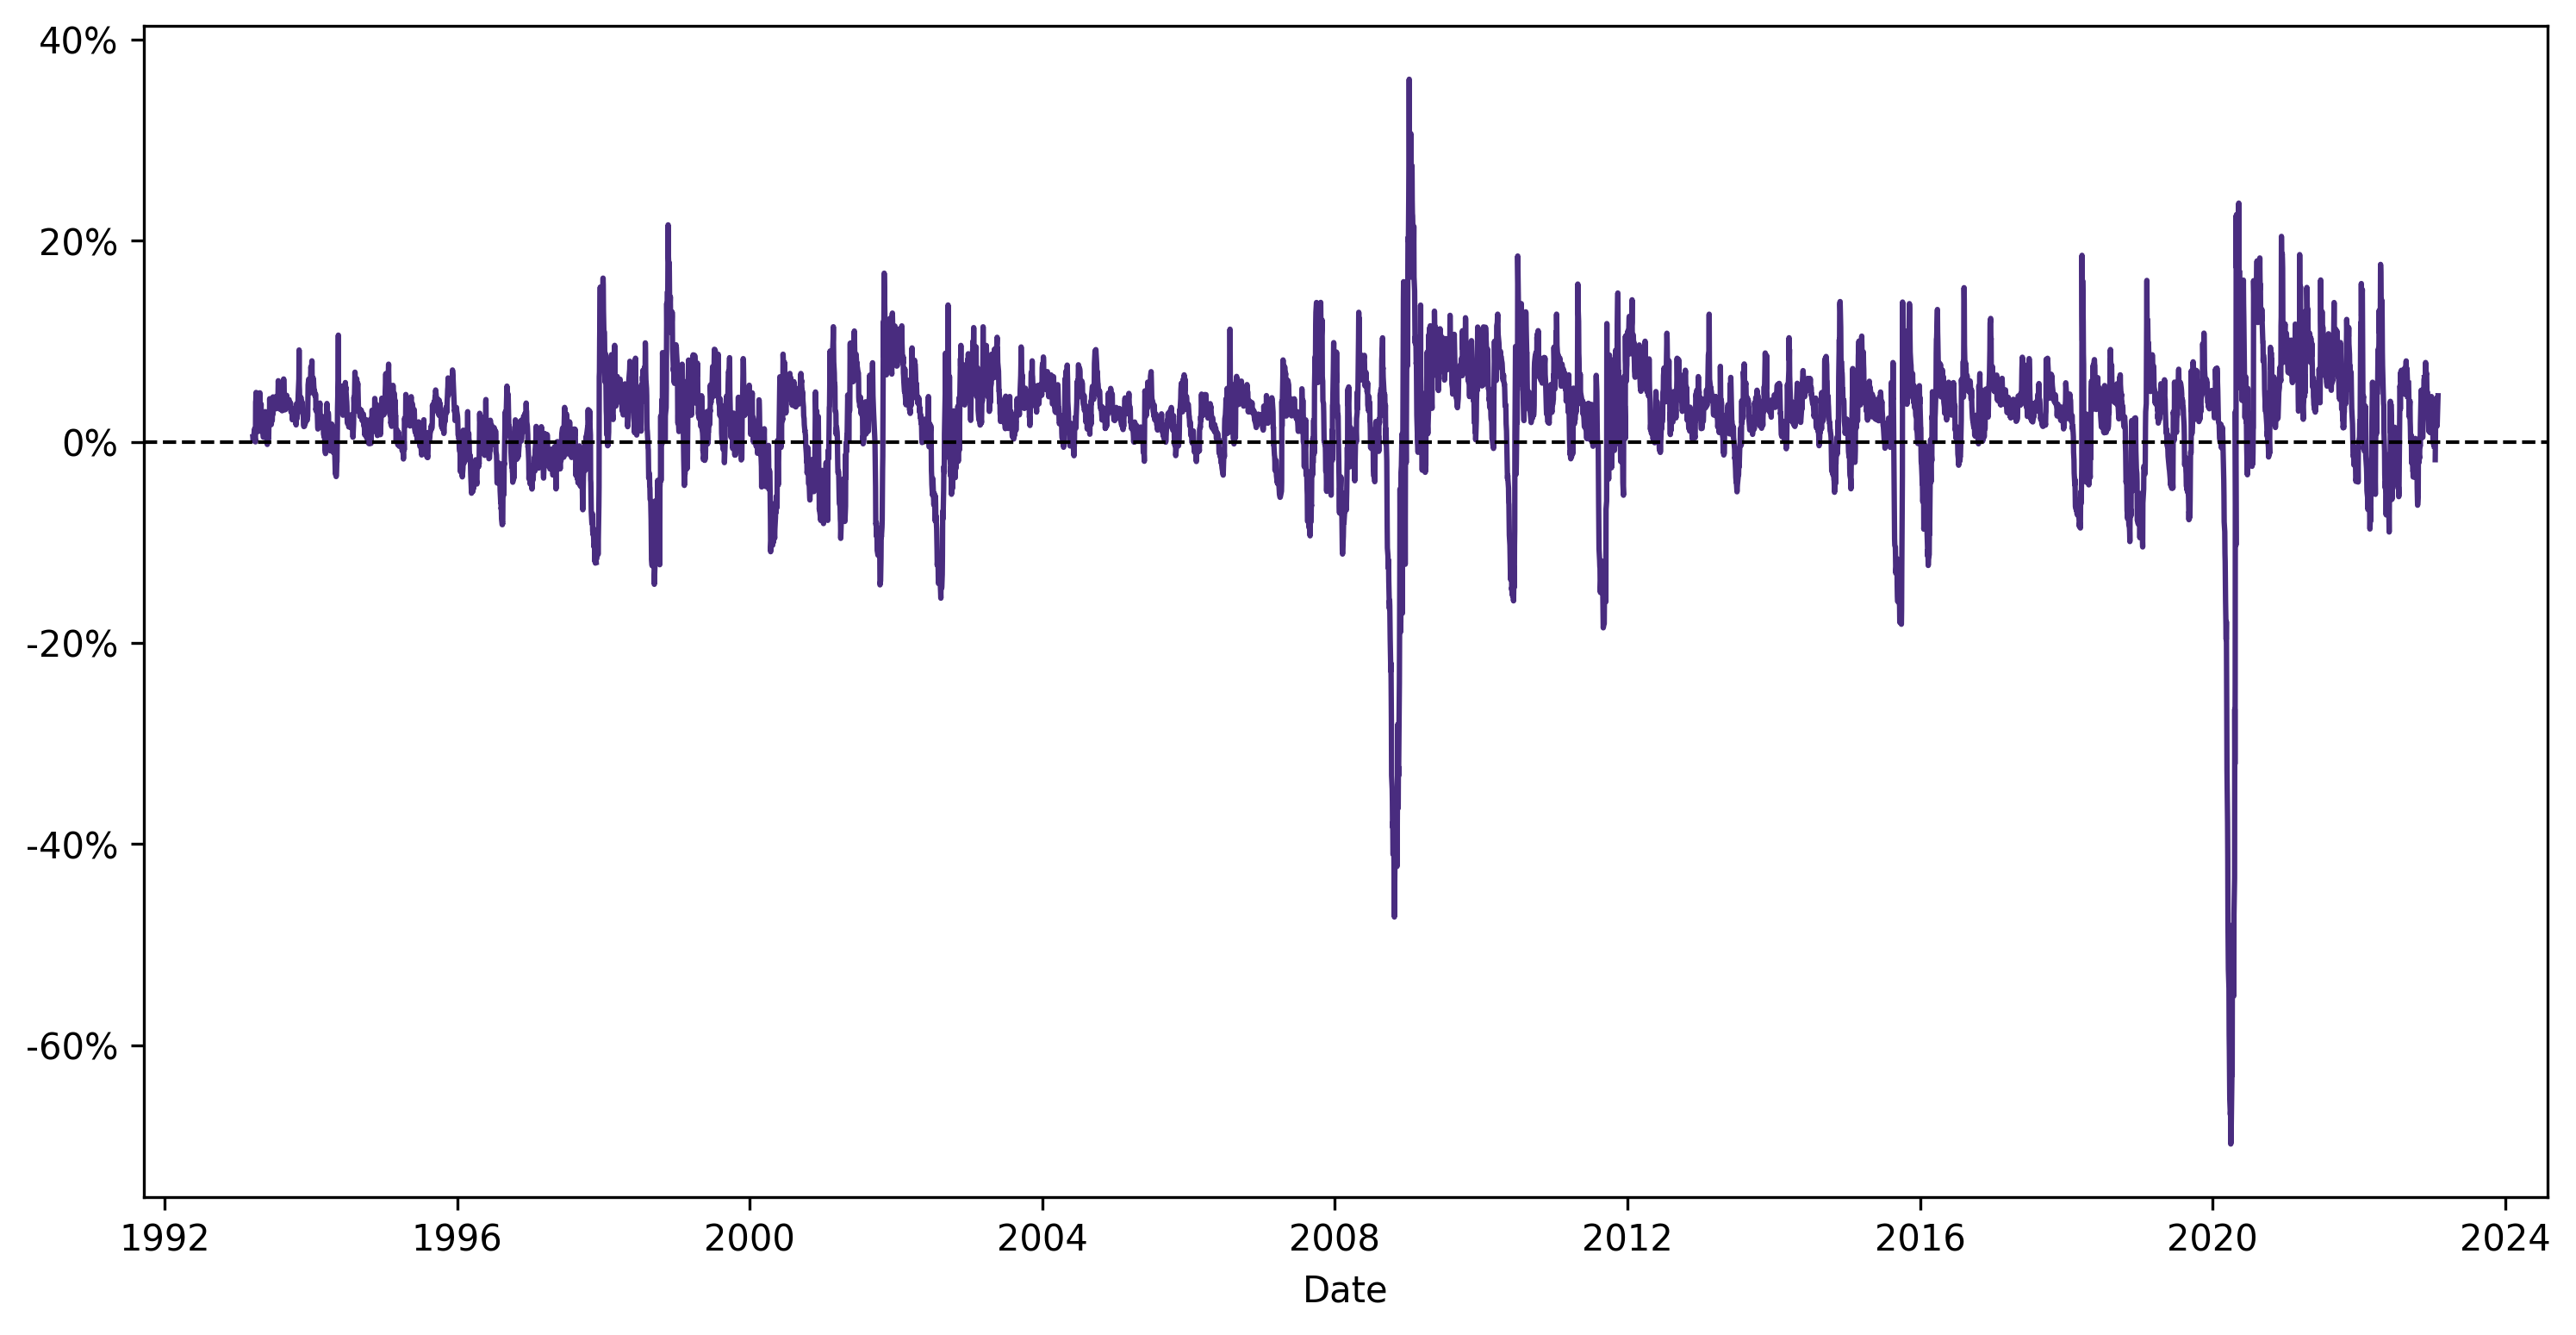
\includegraphics[width=0.95\textwidth]{images/vol_premium.png}
                \end{center}
                \caption{Volatility Risk Premium}
                \label{fig:}
            \end{small}
        \end{figure}
    \end{solution}
\end{enumerate}

\newpage
$ $\clearpage
\bibliography{__references__}
\bibliographystyle{abbrvnat}
\end{document}